\chapter{Market making}
\label{chap:market_making}
A Market Maker (MM) seeks to maximize their terminal wealth by engaging in trading activities through the use of limit orders. In a dealership market(we consider this situation) the MM has the freedom to set the quotes on their platforms. However, the challenge lies in the risk that customers might opt for another dealer who offers more convenient terms.\\
In a Limit Order Book (LOB) market, the strategy needs to account for the presence of other limit orders within the LOB. Failing to consider this can result in an extremely low probability of having orders executed.\\
Similar to any uninformed liquidity provider, the MM faces the risk of adverse selection by informed investors.\\
Even if the flow of investors is not driven by informed trading, there is an additional risk associated with accumulating a large inventory of securities. The key tool at the disposal of the MM is the relationship between the posted prices and the rate at which orders arrive:
\begin{itemize}
	\item By lowering the ask price, the MM can attract more buyers, while raising the ask price, the MM may attract fewer buyers.\\
	\item Lowering the bid price could result in fewer sellers, while raising the bid price may attract more sellers.
\end{itemize}
These adjustments in the posted prices allow the MM to manage and influence trading activity.
\section{Garman model (1976)}
Assume that $\lambda^{Buy}(Ask) = \lambda^{Sell}(Bid)$that is, supply and demand balance (on average).
\begin{center}
	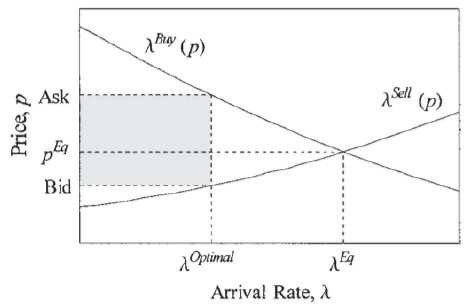
\includegraphics[width=0.5\textwidth]{picture/(23)bid_ask_garman.png}
\end{center}
The prots are dened by the shaded rectangle and the market maker sets the bid and ask to maximize this area.\\
If the market maker sets the Bid and Ask once for all, the holdings of stock follow a zero-drift random walk. Cash holdings follow a positive-drift random walk (due to the turn). Garman points out that in this case, the dealer is eventually ruined with probability one.\\
Need to change the bid and ask quotes to elicit an expected imbalance of buy and sell orders to push their inventories in the direction of their preferred long-run position.\\
Let consider:
\[
\lambda^{buy} = Ae^{-\kappa(S^a-S)} \qquad \lambda^{sell} = Ae^{-\kappa(S-S^b)}
\]
where $S^a$ e $S^b$ are the ask and bid price and $S$ is the equilibrium price, so that:
\[
S^a = S - \frac{1}{\kappa} \ln \frac{\lambda^{buy}}{A} \qquad S^b = S - \frac{1}{\kappa} \ln \frac{\lambda^{sell}}{A}
\]
when $\lambda^{buy} = \lambda^{sell} \equiv \lambda$, profit is:
\[
\text{Profit} = \lambda = \lambda(S^a - S^b) = - \frac{2}{\kappa}\lambda \ln \frac{\lambda}{A}
\]
Profit is maximal if $\lambda = Ae^{-1}$, so the spread is:
\[
\text{Spread} = S_a - S_b = \frac{2}{\kappa}
\]
\newpage
\section{Avellaneda-Stoikov model}
\begin{mysetting}[Avellaneda-Stoikov model]
\begin{itemize}
	\item 	The reference price $S_t$ is modeled by a Brownian dynamics:
	\[
	S_t = \sigma dW_t
	\]
	\item Bid and ask quotes are modeled by $S_t^a$ and $S_t^b$
	\item $(N_t^b)_t$ and $(N_t^a)_t$ are two point processes modeling the number of assets that have
	been respectively bought and sold.
	\item The MM's inventory is:
	\[
	q_t = N_t^b - N_t^a
	\]
	\item The intensity process of $(N_t^b)_t$ and $(N_t^a)_t$  are denoted by $(\lambda_t^b)_t$ and $(\lambda_t^a)_t$
	\[
	(\lambda_t^b)_t = \Lambda^b (\delta_t^b)1_{q_- < Q} \qquad (\lambda_t^a)_t = \Lambda^a (\delta_t^a)1_{q_- < -Q}
	\]
	where:
	\[
	\delta_t^a = S_t - S_t^b \qquad \delta_t^b = S_t^a - S_t 
	\]
where $\Lambda^b$ and $\Lambda^a$ are two positive nonincreasing functions. 
\item $Q\in \mathbb{N}$ is the maximum authorized invetory. MM stops posting a bid(ask) when \\$q_t =Q(q_t = - Q)$
\item We assume:
\[
\Lambda^b(\delta) = \Lambda^a(\delta)=Ae^{-\kappa\delta}
\]
where $A>0$ is the liquidity of the asset and $\kappa >0$ characterises the price sensitivity of the market participants.
\end{itemize}
\end{mysetting}
The amount of cash $dX_t = S_t^a dN^a_t-S_t^bdN_t^b = (S_t + \delta_t^a)dN_t^a - (S_t - \delta_t^b)dN_t^b $.\\
The goal of MM is to maximize the expected (CARA) utility functionmn at some determined time horizon $T$, s.t:
\[
\expected{-\exp\{-\gamma(X_T + q_TS_t - l(q_T))\}}
\]
the term $l(q_t)$represents a penalization for the final inventory.\\
The solution requires tolls of stochastic optimization and we have to solve the associated Hamilton-Jacobi-Bellman equation. The system can be solvend numerically or exactly.
\newpage
\begin{mytheorem}[Avellaneda-Stoikov model solution]
	The optimal bid and quotes of the market maker in Avellaneda-Stoikov model are:
	\begin{align*}
		& S^b(t,S,q) = S - \frac{1}{\kappa} \ln \left( \frac{v_q(t)}{v_{q+1}(t)}\right) - \frac{1}{\gamma} \ln\left(1 + \frac{\gamma}{\kappa}\right) \\
		& S^a(t,S,q) = S - \frac{1}{\kappa} \ln \left( \frac{v_q(t)}{v_{q-1}(t)}\right) - \frac{1}{\gamma} \ln\left(1 + \frac{\gamma}{\kappa}\right)
	\end{align*}
\end{mytheorem}
Some general comment:
\begin{itemize}
	\item In some situations it might look unnatural to consider a finite terminal time $T$
	\item when $T \to \infty$ the optimal spread is approximated by:
	\[
	\text{Spread} = S^a - S^b \simeq \frac{2}{\gamma} \ln \left(1 + \frac{\lambda}{\gamma}\right) + \sqrt{\frac{\sigma^2 \gamma}{2\kappa A}\left(1 + \frac{\gamma}{\kappa}\right)^{1 + \frac{\kappa}{\gamma}}}
	\]
	which does not depend on the inventory $q$
	\item The skewness of the strategy is:
	\[
	(S - S^b) - (S^a - S) \propto q
	\] 
	\item The MM faces two risks: transiction uncertainty and price risk
	\item if $\sigma = 0$, there is a spread:
	\[
	\text{Spread} \simeq \frac{2}{\gamma} \ln \left(1 + \frac{\gamma}{\kappa}\right) \xrightarrow[]{\gamma \to 0} \frac{2}{\kappa}
	\]
	that is a decreasing function of $\gamma$. Spread is $2/\kappa$ when $\gamma = 0$ even if $\sigma \neq 0$
	\item the skewness increases with $\sigma$ and $\gamma$
\end{itemize}
Limitation of this model are:
\begin{itemize}
	\item The model can be enriched by adding short term $\alpha$, price drift, etc.
	\item Price is a continuous variable
	\item It is hard to apply in LOB market
	\item The function $\Gamma$ are exponential
	\item It considers only one asset
\end{itemize}